
%% bare_conf.tex
%% V1.3
%% 2007/01/11
%% by Michael Shell
%% See:
%% http://www.michaelshell.org/
%% for current contact information.
%%
%% This is a skeleton file demonstrating the use of IEEEtran.cls
%% (requires IEEEtran.cls version 1.7 or later) with an IEEE conference paper.
%%
%% Support sites:
%% http://www.michaelshell.org/tex/ieeetran/
%% http://www.ctan.org/tex-archive/macros/latex/contrib/IEEEtran/
%% and
%% http://www.ieee.org/

%%*************************************************************************
%% Legal Notice:
%% This code is offered as-is without any warranty either expressed or
%% implied; without even the implied warranty of MERCHANTABILITY or
%% FITNESS FOR A PARTICULAR PURPOSE! 
%% User assumes all risk.
%% In no event shall IEEE or any contributor to this code be liable for
%% any damages or losses, including, but not limited to, incidental,
%% consequential, or any other damages, resulting from the use or misuse
%% of any information contained here.
%%
%% All comments are the opinions of their respective authors and are not
%% necessarily endorsed by the IEEE.
%%
%% This work is distributed under the LaTeX Project Public License (LPPL)
%% ( http://www.latex-project.org/ ) version 1.3, and may be freely used,
%% distributed and modified. A copy of the LPPL, version 1.3, is included
%% in the base LaTeX documentation of all distributions of LaTeX released
%% 2003/12/01 or later.
%% Retain all contribution notices and credits.
%% ** Modified files should be clearly indicated as such, including  **
%% ** renaming them and changing author support contact information. **
%%
%% File list of work: IEEEtran.cls, IEEEtran_HOWTO.pdf, bare_adv.tex,
%%                    bare_conf.tex, bare_jrnl.tex, bare_jrnl_compsoc.tex
%%*************************************************************************

% *** Authors should verify (and, if needed, correct) their LaTeX system  ***
% *** with the testflow diagnostic prior to trusting their LaTeX platform ***
% *** with production work. IEEE's font choices can trigger bugs that do  ***
% *** not appear when using other class files.                            ***
% The testflow support page is at:
% http://www.michaelshell.org/tex/testflow/



% Note that the a4paper option is mainly intended so that authors in
% countries using A4 can easily print to A4 and see how their papers will
% look in print - the typesetting of the document will not typically be
% affected with changes in paper size (but the bottom and side margins will).
% Use the testflow package mentioned above to verify correct handling of
% both paper sizes by the user's LaTeX system.
%
% Also note that the "draftcls" or "draftclsnofoot", not "draft", option
% should be used if it is desired that the figures are to be displayed in
% draft mode.
%
\documentclass[conference]{IEEEtran}


% Add the compsoc option for Computer Society conferences.
%
% If IEEEtran.cls has not been installed into the LaTeX system files,
% manually specify the path to it like:
% \documentclass[conference]{../sty/IEEEtran}





% Some very useful LaTeX packages include:
% (uncomment the ones you want to load)


% *** MISC UTILITY PACKAGES ***
%
%\usepackage{ifpdf}
% Heiko Oberdiek's ifpdf.sty is very useful if you need conditional
% compilation based on whether the output is pdf or dvi.
% usage:
% \ifpdf
%   % pdf code
% \else
%   % dvi code
% \fi
% The latest version of ifpdf.sty can be obtained from:
% http://www.ctan.org/tex-archive/macros/latex/contrib/oberdiek/
% Also, note that IEEEtran.cls V1.7 and later provides a builtin
% \ifCLASSINFOpdf conditional that works the same way.
% When switching from latex to pdflatex and vice-versa, the compiler may
% have to be run twice to clear warning/error messages.






% *** CITATION PACKAGES ***
%
%\usepackage{cite}
% cite.sty was written by Donald Arseneau
% V1.6 and later of IEEEtran pre-defines the format of the cite.sty package
% \cite{} output to follow that of IEEE. Loading the cite package will
% result in citation numbers being automatically sorted and properly
% "compressed/ranged". e.g., [1], [9], [2], [7], [5], [6] without using
% cite.sty will become [1], [2], [5]--[7], [9] using cite.sty. cite.sty's
% \cite will automatically add leading space, if needed. Use cite.sty's
% noadjust option (cite.sty V3.8 and later) if you want to turn this off.
% cite.sty is already installed on most LaTeX systems. Be sure and use
% version 4.0 (2003-05-27) and later if using hyperref.sty. cite.sty does
% not currently provide for hyperlinked citations.
% The latest version can be obtained at:
% http://www.ctan.org/tex-archive/macros/latex/contrib/cite/
% The documentation is contained in the cite.sty file itself.






% *** GRAPHICS RELATED PACKAGES ***
%
\usepackage{listings}
\usepackage{hyperref}
\usepackage{graphicx}
\graphicspath{{./images/}}
\DeclareGraphicsExtensions{.eps}

\ifCLASSINFOpdf
  %\usepackage[pdftex]{graphicx}
  % declare the path(s) where your graphic files are
  % \graphicspath{{../pdf/}{../jpeg/}}
  % and their extensions so you won't have to specify these with
  % every instance of \includegraphics
  % \DeclareGraphicsExtensions{.pdf,.jpeg,.png}
\else
  % or other class option (dvipsone, dvipdf, if not using dvips). graphicx
  % will default to the driver specified in the system graphics.cfg if no
  % driver is specified.
  %\usepackage[dvips]{graphicx}
  % declare the path(s) where your graphic files are
  % \graphicspath{{../eps/}}
  % and their extensions so you won't have to specify these with
  % every instance of \includegraphics
  % \DeclareGraphicsExtensions{.eps}
\fi
% graphicx was written by David Carlisle and Sebastian Rahtz. It is
% required if you want graphics, photos, etc. graphicx.sty is already
% installed on most LaTeX systems. The latest version and documentation can
% be obtained at: 
% http://www.ctan.org/tex-archive/macros/latex/required/graphics/
% Another good source of documentation is "Using Imported Graphics in
% LaTeX2e" by Keith Reckdahl which can be found as epslatex.ps or
% epslatex.pdf at: http://www.ctan.org/tex-archive/info/
%
% latex, and pdflatex in dvi mode, support graphics in encapsulated
% postscript (.eps) format. pdflatex in pdf mode supports graphics
% in .pdf, .jpeg, .png and .mps (metapost) formats. Users should ensure
% that all non-photo figures use a vector format (.eps, .pdf, .mps) and
% not a bitmapped formats (.jpeg, .png). IEEE frowns on bitmapped formats
% which can result in "jaggedy"/blurry rendering of lines and letters as
% well as large increases in file sizes.
%
% You can find documentation about the pdfTeX application at:
% http://www.tug.org/applications/pdftex





% *** MATH PACKAGES ***
%
%\usepackage[cmex10]{amsmath}
% A popular package from the American Mathematical Society that provides
% many useful and powerful commands for dealing with mathematics. If using
% it, be sure to load this package with the cmex10 option to ensure that
% only type 1 fonts will utilized at all point sizes. Without this option,
% it is possible that some math symbols, particularly those within
% footnotes, will be rendered in bitmap form which will result in a
% document that can not be IEEE Xplore compliant!
%
% Also, note that the amsmath package sets \interdisplaylinepenalty to 10000
% thus preventing page breaks from occurring within multiline equations. Use:
%\interdisplaylinepenalty=2500
% after loading amsmath to restore such page breaks as IEEEtran.cls normally
% does. amsmath.sty is already installed on most LaTeX systems. The latest
% version and documentation can be obtained at:
% http://www.ctan.org/tex-archive/macros/latex/required/amslatex/math/





% *** SPECIALIZED LIST PACKAGES ***
%
%\usepackage{algorithmic}
% algorithmic.sty was written by Peter Williams and Rogerio Brito.
% This package provides an algorithmic environment fo describing algorithms.
% You can use the algorithmic environment in-text or within a figure
% environment to provide for a floating algorithm. Do NOT use the algorithm
% floating environment provided by algorithm.sty (by the same authors) or
% algorithm2e.sty (by Christophe Fiorio) as IEEE does not use dedicated
% algorithm float types and packages that provide these will not provide
% correct IEEE style captions. The latest version and documentation of
% algorithmic.sty can be obtained at:
% http://www.ctan.org/tex-archive/macros/latex/contrib/algorithms/
% There is also a support site at:
% http://algorithms.berlios.de/index.html
% Also of interest may be the (relatively newer and more customizable)
% algorithmicx.sty package by Szasz Janos:
% http://www.ctan.org/tex-archive/macros/latex/contrib/algorithmicx/




% *** ALIGNMENT PACKAGES ***
%
%\usepackage{array}
% Frank Mittelbach's and David Carlisle's array.sty patches and improves
% the standard LaTeX2e array and tabular environments to provide better
% appearance and additional user controls. As the default LaTeX2e table
% generation code is lacking to the point of almost being broken with
% respect to the quality of the end results, all users are strongly
% advised to use an enhanced (at the very least that provided by array.sty)
% set of table tools. array.sty is already installed on most systems. The
% latest version and documentation can be obtained at:
% http://www.ctan.org/tex-archive/macros/latex/required/tools/


%\usepackage{mdwmath}
%\usepackage{mdwtab}
% Also highly recommended is Mark Wooding's extremely powerful MDW tools,
% especially mdwmath.sty and mdwtab.sty which are used to format equations
% and tables, respectively. The MDWtools set is already installed on most
% LaTeX systems. The lastest version and documentation is available at:
% http://www.ctan.org/tex-archive/macros/latex/contrib/mdwtools/


% IEEEtran contains the IEEEeqnarray family of commands that can be used to
% generate multiline equations as well as matrices, tables, etc., of high
% quality.


%\usepackage{eqparbox}
% Also of notable interest is Scott Pakin's eqparbox package for creating
% (automatically sized) equal width boxes - aka "natural width parboxes".
% Available at:
% http://www.ctan.org/tex-archive/macros/latex/contrib/eqparbox/





% *** SUBFIGURE PACKAGES ***
%\usepackage[tight,footnotesize]{subfigure}
% subfigure.sty was written by Steven Douglas Cochran. This package makes it
% easy to put subfigures in your figures. e.g., "Figure 1a and 1b". For IEEE
% work, it is a good idea to load it with the tight package option to reduce
% the amount of white space around the subfigures. subfigure.sty is already
% installed on most LaTeX systems. The latest version and documentation can
% be obtained at:
% http://www.ctan.org/tex-archive/obsolete/macros/latex/contrib/subfigure/
% subfigure.sty has been superceeded by subfig.sty.



%\usepackage[caption=false]{caption}
%\usepackage[font=footnotesize]{subfig}
% subfig.sty, also written by Steven Douglas Cochran, is the modern
% replacement for subfigure.sty. However, subfig.sty requires and
% automatically loads Axel Sommerfeldt's caption.sty which will override
% IEEEtran.cls handling of captions and this will result in nonIEEE style
% figure/table captions. To prevent this problem, be sure and preload
% caption.sty with its "caption=false" package option. This is will preserve
% IEEEtran.cls handing of captions. Version 1.3 (2005/06/28) and later 
% (recommended due to many improvements over 1.2) of subfig.sty supports
% the caption=false option directly:
%\usepackage[caption=false,font=footnotesize]{subfig}
%
% The latest version and documentation can be obtained at:
% http://www.ctan.org/tex-archive/macros/latex/contrib/subfig/
% The latest version and documentation of caption.sty can be obtained at:
% http://www.ctan.org/tex-archive/macros/latex/contrib/caption/




% *** FLOAT PACKAGES ***
%
%\usepackage{fixltx2e}
% fixltx2e, the successor to the earlier fix2col.sty, was written by
% Frank Mittelbach and David Carlisle. This package corrects a few problems
% in the LaTeX2e kernel, the most notable of which is that in current
% LaTeX2e releases, the ordering of single and double column floats is not
% guaranteed to be preserved. Thus, an unpatched LaTeX2e can allow a
% single column figure to be placed prior to an earlier double column
% figure. The latest version and documentation can be found at:
% http://www.ctan.org/tex-archive/macros/latex/base/



%\usepackage{stfloats}
% stfloats.sty was written by Sigitas Tolusis. This package gives LaTeX2e
% the ability to do double column floats at the bottom of the page as well
% as the top. (e.g., "\begin{figure*}[!b]" is not normally possible in
% LaTeX2e). It also provides a command:
%\fnbelowfloat
% to enable the placement of footnotes below bottom floats (the standard
% LaTeX2e kernel puts them above bottom floats). This is an invasive package
% which rewrites many portions of the LaTeX2e float routines. It may not work
% with other packages that modify the LaTeX2e float routines. The latest
% version and documentation can be obtained at:
% http://www.ctan.org/tex-archive/macros/latex/contrib/sttools/
% Documentation is contained in the stfloats.sty comments as well as in the
% presfull.pdf file. Do not use the stfloats baselinefloat ability as IEEE
% does not allow \baselineskip to stretch. Authors submitting work to the
% IEEE should note that IEEE rarely uses double column equations and
% that authors should try to avoid such use. Do not be tempted to use the
% cuted.sty or midfloat.sty packages (also by Sigitas Tolusis) as IEEE does
% not format its papers in such ways.





% *** PDF, URL AND HYPERLINK PACKAGES ***
%
%\usepackage{url}
% url.sty was written by Donald Arseneau. It provides better support for
% handling and breaking URLs. url.sty is already installed on most LaTeX
% systems. The latest version can be obtained at:
% http://www.ctan.org/tex-archive/macros/latex/contrib/misc/
% Read the url.sty source comments for usage information. Basically,
% \url{my_url_here}.





% *** Do not adjust lengths that control margins, column widths, etc. ***
% *** Do not use packages that alter fonts (such as pslatex).         ***
% There should be no need to do such things with IEEEtran.cls V1.6 and later.
% (Unless specifically asked to do so by the journal or conference you plan
% to submit to, of course. )


% correct bad hyphenation here
%\hyphenation{op-tical net-works semi-conduc-tor}


\begin{document}
%
% paper title
% can use linebreaks \\ within to get better formatting as desired
\title{BlockPy: From Interest to Usefulness in a Block-based, Educational Environment}


% author names and affiliations
% use a multiple column layout for up to three different
% affiliations
\author{\IEEEauthorblockN{Austin Cory Bart, Eli Tilevich, Clifford A. Shaffer, Dennis Kafura}
\IEEEauthorblockA{Computer Science\\
Virginia Tech\\
Blacksburg, VA 24060\\
\{acbart, tilevich, shaffer, kafura\}@vt.edu}
}

% conference papers do not typically use \thanks and this command
% is locked out in conference mode. If really needed, such as for
% the acknowledgment of grants, issue a \IEEEoverridecommandlockouts
% after \documentclass

% for over three affiliations, or if they all won't fit within the width
% of the page, use this alternative format:
% 
%\author{\IEEEauthorblockN{Michael Shell\IEEEauthorrefmark{1},
%Homer Simpson\IEEEauthorrefmark{2},
%James Kirk\IEEEauthorrefmark{3}, 
%Montgomery Scott\IEEEauthorrefmark{3} and
%Eldon Tyrell\IEEEauthorrefmark{4}}
%\IEEEauthorblockA{\IEEEauthorrefmark{1}School of Electrical and Computer Engineering\\
%Georgia Institute of Technology,
%Atlanta, Georgia 30332--0250\\ Email: see http://www.michaelshell.org/contact.html}
%\IEEEauthorblockA{\IEEEauthorrefmark{2}Twentieth Century Fox, Springfield, USA\\
%Email: homer@thesimpsons.com}
%\IEEEauthorblockA{\IEEEauthorrefmark{3}Starfleet Academy, San Francisco, California 96678-2391\\
%Telephone: (800) 555--1212, Fax: (888) 555--1212}
%\IEEEauthorblockA{\IEEEauthorrefmark{4}Tyrell Inc., 123 Replicant Street, Los Angeles, California 90210--4321}}




% use for special paper notices
%\IEEEspecialpapernotice{(Invited Paper)}




% make the title area
\maketitle


\begin{abstract}
%\boldmath
As block-based environments are used for more mature audiences, the environments must mature themselves.
Based on holistic theories of academic motivation, this means making the environment present itself as both Interesting \textit{and} Useful, without sacricing pedagogical power and scaffolding.
We present Data Science as a potential context that satisfies all of these constraints, and describe our new block-based programming environment for education that supports Data Science from day one: BlockPy, available at \url{http://think.cs.vt.edu/blockpy/}.
Blockpy features a number of powerful, authentic features meant to promote transfer for students as they progress.
This includes Mutual Language Translation and interactive feedback, but also powerful tools for getting real-world data and visualizing it.
As we have developed the tool, we have identified a number of major research questions that should be answered in order to determine the validity of our hypothesis and the potential of our approach: in particular, how can this environment and context support educators and diverse learners as they progress into conventional environments.
\end{abstract}
% IEEEtran.cls defaults to using nonbold math in the Abstract.
% This preserves the distinction between vectors and scalars. However,
% if the conference you are submitting to favors bold math in the abstract,
% then you can use LaTeX's standard command \boldmath at the very start
% of the abstract to achieve this. Many IEEE journals/conferences frown on
% math in the abstract anyway.

% no keywords




% For peer review papers, you can put extra information on the cover
% page as needed:
% \ifCLASSOPTIONpeerreview
% \begin{center} \bfseries EDICS Category: 3-BBND \end{center}
% \fi
%
% For peerreview papers, this IEEEtran command inserts a page break and
% creates the second title. It will be ignored for other modes.
\IEEEpeerreviewmaketitle



\section{Problem}

How do we bring introductory computing to mature, domain-identified undergraduates, who have concerns for both their own self-efficacy and for the value in learning computing?
Many universities are now defining core credit hours in subjects such as ``Computational Thinking'', introductory computer science classes meant for solving interdisciplinary problems using some degree of programming.
This means that universities now have students of every different discipline and background taking a programming course.
Students with a clearly domain-identified interest (i.e. their major) may view non-major courses with doubt and suspicion -- what does this have to offer them, and why should they engage?

Our position is that, in order to fully engage all undergraduate students, an introductory programming environment should be both \textit{interesting} and \textit{useful}, while still promoting \textit{success}.
Critically, this means that the environment should enable working with a context that students relate to, enjoy, and helps them solve useful problems.
Further, they should feel that the material that they're learning will help them to transition to more authentic, serious problem-solving of real programming environments.
These changes cannot come at the cost of the pedagogically valuable scaffolding, but instead should provide new opportunities for students' learning.

\subsection{Existing Solutions}

Although Block-based environments like Scratch and Snap! have already been successful with high-school students, they may not be suitable for more mature but diverse populations.
In addition to side-stepping syntax headaches, Snap! and Scratch environments make it easier to get working with their motivating educational context, such as game and animation design, robots, or media computation, because they expose the range of actions afforded by the context (e.g., a ``draw a circle'' block for media computation) and support the experiences directly (e.g., a drawing canvas embedded within the environment).
These contexts can be very popular with certain students: young male children usually enjoy creating games, for example, so game and animation design is a very compelling hook.
However, many students at the undergraduate level may doubt the usefulness of the environment, as they consider it a toy rather than a useful tool, not only because of the puzzle-piece metaphor they utilize, but also for the evironments' contexts.

\subsection{A New Solution: Data Science}

We submit \textit{Data Science Exploration} as an educational context that block-based environments should support as a first-class citizen, similar to how Snap! and Scratch support game design.
Data Science for Introductory Computing is a growing movement, with many instructors recognizing the inherent value ~\cite{Anderson, Sullivan:2013}
Data science provides an authentic, useful context for every kind of students, since exploring data-oriented problems is something that almost all fields are beginning to find relevant~\cite{Layman:2007, Social-good}.
Additionally, it is readily possible to find data sources that connect to the world around the student and their past experiences, establishing a sense of personalized interest.
When students inevitably ask, ``What am I going to be using this for?'', it is possible to point to well-defined data problems in their field requiring computation.
This does not mean that we are creating an end-user programming environment for data science, however, but an educational environment that allows students to learn computing principles through the context of data science (similar to how Scratch is meant to learn programming, rather than to learn game design).

\begin{figure*}[t]
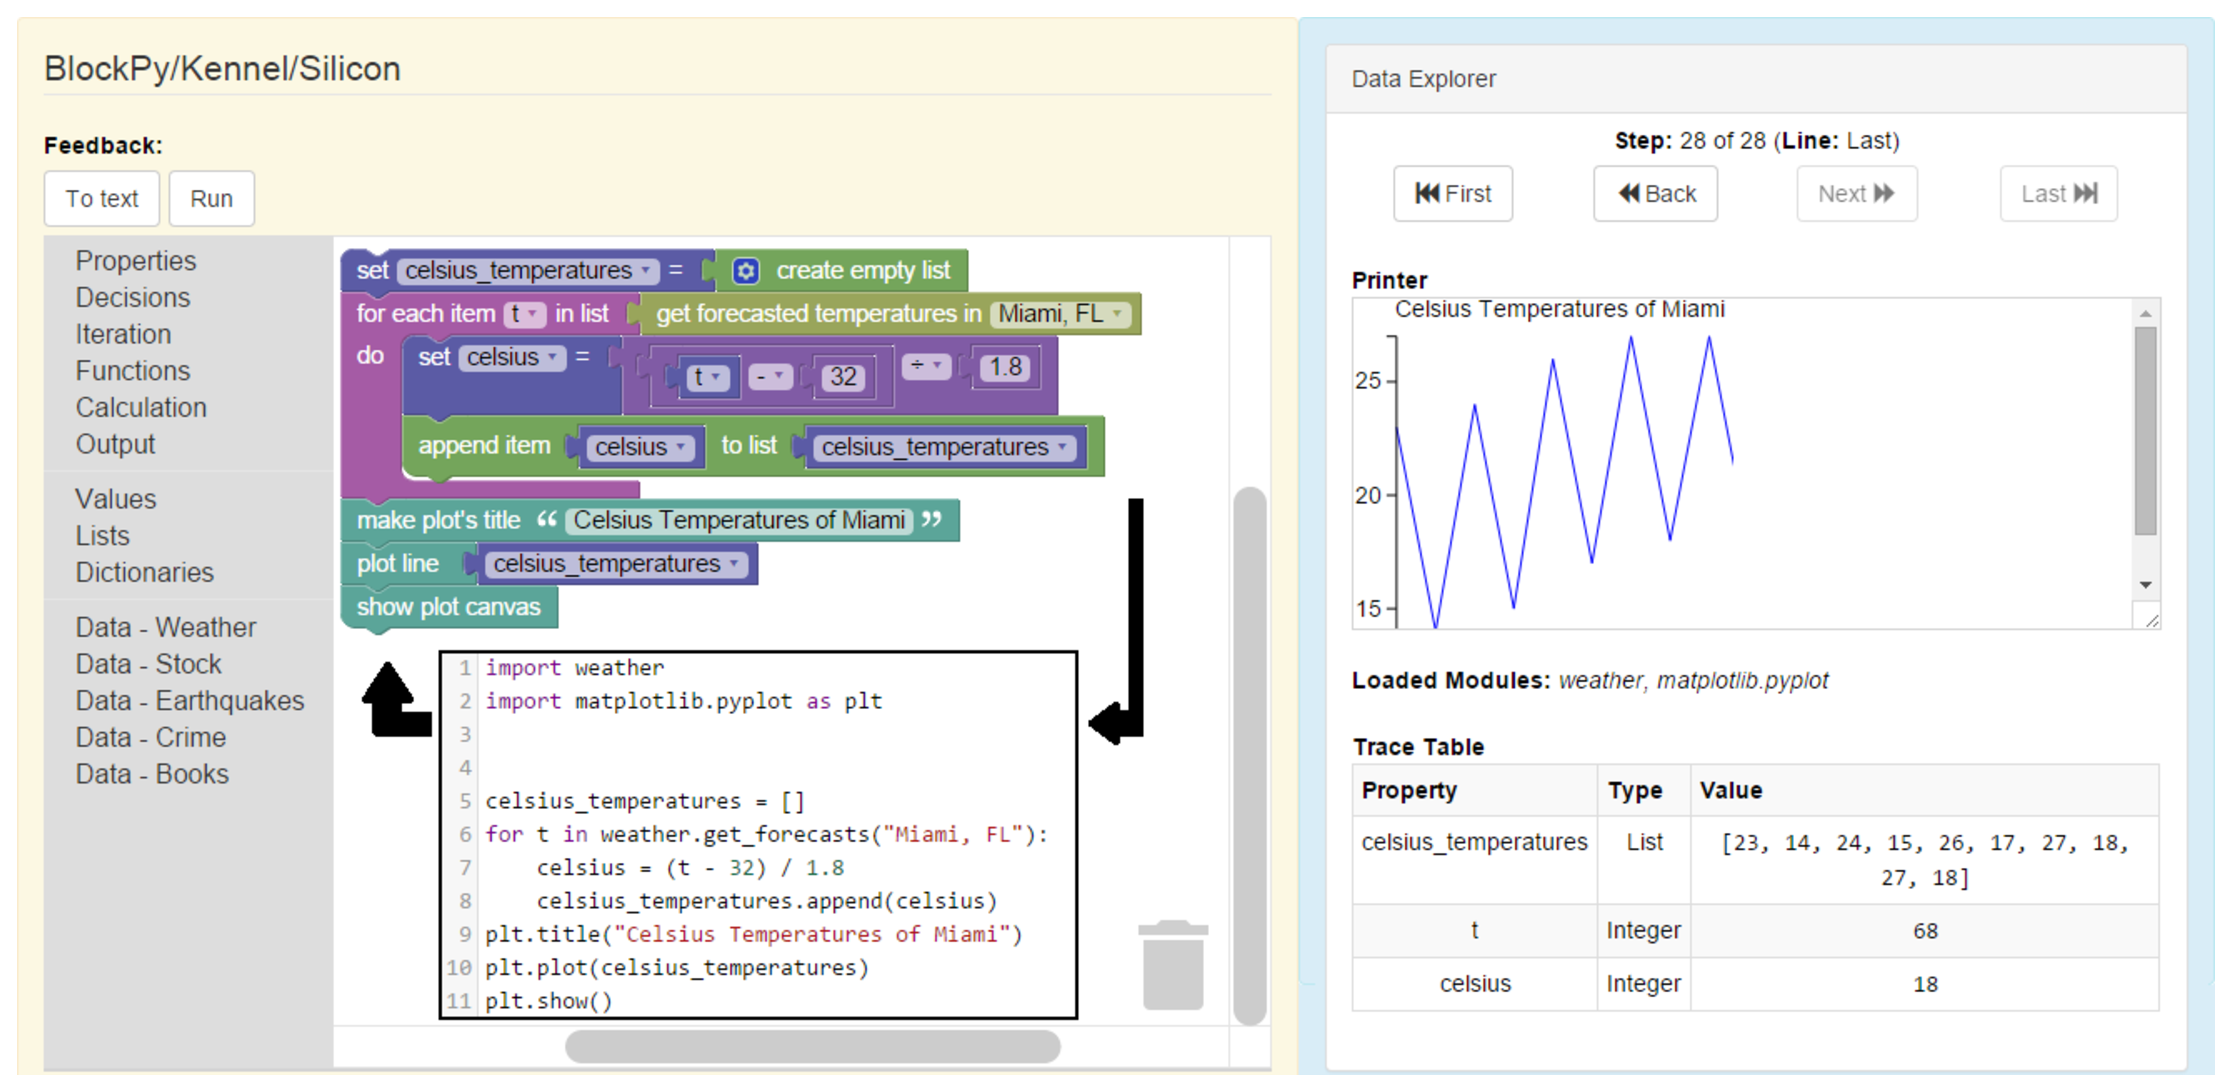
\includegraphics[width=\linewidth, keepaspectratio]{full-kennel.eps}
\caption{A complete representation of BlockPy (\url{http://think.cs.vt.edu/blockpy/} )}
\label{fig-blockpy-full}
\end{figure*}

\subsection{Academic Motivation and Blocks}

The prior research on block-based environments in undergraduate settings sheds some light on the limitations of existing environments for those populations.
Mishra conducted a two-week intervention in an introductory course where students worked with Scratch before they began working with Java, reporting positive outcomes in both learning and engagement~\cite{Mishra}.
However, although the sample population was quite large (N=450), the students do not represent the typical body of a university: they were non-CS engineering majors, 88\% male, and ``highest ranked'' in ``mathematics, physics, and chemistry''.
The students did vary greatly on prior programming performance, but their other demographics suggest that they have rather uniform motivational concerns, compared to the general undergraduate population.
In particular, the perception survey revealed that many students cited the game design context afforded by Scratch as a major motivating factor: ``[I am] thrilled to be able to code complex games'' and ``[coding] games helped increase my interest, [...], there was lot of room for experimentation.''
These students valued the game design component because it was interesting to them, but not because they saw it as useful to their careers.
It is unclear how more diverse students would react to this environment.

In our research project, we use the MUSIC Model of Academic Motivation\cite{jones-description} in order to explain the different ways students become engaged. Specifically, this model differentiates between five components of motivation: \textbf{eMpowerment}, the control that a student feels that they have over their learning experience; \textbf{Usefulness}, the expectation of the student that the material will be valuable to their short- and long-term goals; \textbf{Success}, the student's self-efficacy; \textbf{Interest}, the situational and dispostional value the student's feels; and \textbf{Caring}, the students perception of their professor's and classmates attitudes toward them.
We apply this theory to describe existing game-based programming environments as providing Interest to certain populations, but limited opportunities for Usefulness.
We suggest that more students (and more typical students) can be better served with a context that supports all five dimensions and, in particular, both general Interest and Usefulness.
To that end, we have created a new block-based environment with this theory in mind.

\section{BlockPy}
	
In this section, we concretely describe our work on a new web-based, dual text/block environment:
\textbf{BlockPy}, a beginner-friendly programming environment that scaffolds the learner into a more mature environment while supporting a sense of Usefulness up-front.
Internally, BlockPy uses a modified version of the open-source Blockly library to provide a block editor, a modified version of the open-source Skulpt library to execute Python code client-side, and an unmodified version of the open-source CodeMirror library to provide a text editor.
Figure \ref{fig-blockpy-full} demonstrates the interface: the problem presentation and feedback on the top-left, the dual program representations in the bottom left (via Mutual Language Translation), and the data science dashboard on the right (giving students powerful insight into their programs execution).

\subsection{Data Science as a First-Class Feature}

The code represented in the figure demonstrates the data science API exposed to the student, including blocks and functions to access real-world data sources and to create visualizations.
These data sources include weather forecasts, earthquake reports, and stock feeds.
Data returned from their interface is extremely simple -- usually either primitive (numbers and text) or minimally structured (maps and lists), ensuring that students can begin working with Big Data blocks at the earliest possible points in the course.
In addition to obtaining data, we support the popular MatPlotlib library to provide a set of visualization functions create simple line plots and histograms.
By basing everything around the MatPlotLib API and relying on the Blocks interface for scaffolding, BlockPy seeks to maintain complete compatibility with conventional Python APIs so that all code written is authentic, as opposed to the use of simplified toy APIs in environments like CodeSkulptor.

\subsection{Guided Practice}

BlockPy is not just a code-authoring environment but also a system for guided practice.
Instructors can create problems by writing introductory text and then using an assessment API to define interactive feedback.
Specifically, the instructor can define rules based on students' current code, output, and program state, and gives automatic feedback to the student.
This just-in-time feedback is meant to guide students to success.
Of course, the environment also supports free-form coding experiences, as you would find in traditional programming environments; as the students progress through their introductory experience, short-term feedback can decrease and then fade away.

\subsection{Transfer to Authenticity}

Although some research is working towards creating end-user block-based environments, we view block-based languages as ``Training Wheels'', meant to be faded away.
Work by Weintrop on the transition from Snap to Python analyzes this transition and offers a number of ways to mediate the transfer through programming tools. 
One of the largest findings is that being able to write inline code inside a Block-based language is extremely helpful to students' learning \cite{Weintrop}.
Another approach we support is Mutual Language Translation, devised by Matsuzawa ~\cite{Matsuzawa}, that creates an isomorphic view of students' code as both text and blocks.
These features are meant to transfer students away from blocks towards text.

\subsection{An Example Scenario}

Consider a lesson for students on Iteration.
The instructor could create a problem asking students to find the average temperature in their local city for this week, using the assessment API to construct rules demanding they use iteration blocks.
Students would begin by dragging in a \texttt{Get Temperatures for [city]} block.
If they attempt to run their code at this point, they will be reminded that averaging requires iteration.
As they continue, they can switch between the block and textual view as they feel comfortable.
They can also use the data explorer to step through their code and watch its state change.
Finally, when they successfully print the answer, they are given positive feedback.
	
\section{Research Questions}

Our new programming environment offers a number of affordances to educators, but much of its promise is still unproven.
Beyond just usability testing, we wish to explore questions relating to the nature of using data science in a block environment.
One of the major values of a context is being relatable -- it should be a metaphor for students, helping to build on their prior knowledge. Will the entire undergraduate population find data science to be sufficiently relatable? For instance, some students may possess weak math skills or have low self-efficacy with math. Will they find the necessary mathematics (e.g., finding the average of a list) too confusing?

Along similar lines, how do we quickly introduce students to a given dataset, and make them comfortable manipulating and understanding the data it contains?
What interaction can the students have with the blocks in order to aid this experience?
In the datasets currently supported by the environment, some are ``easier'' than the others: our students had no trouble working with weather data, for instance, but struggled when confronted by stock trading data.
Are some datasets inherently more suitable for introductory experiences?
And just how crucial are students' perceptions of interest and usefulness? 

Of course, our environments' affordances also raise more general questions.
In our own experiences with using a block-based environment to scaffold learners into a serious environment, the transfer can be very rocky.
Some students are eager to start using the text-based environment and do not need to pushed to move away from the blocks.
However, some students may be wary about losing their training wheels and, if left to their own devices, may choose to delay trying out the text-based code.
How do we gracefully transition students to writing text, based on the students' ability level, motivational level, and the course's time table?
How does Mutual Language Translation support and hinder this process?
And how do we provide accurate block-based representations of a dynamic language like Python -- consider the difficulties involved in inferring whether a variable block has the appropriate type to be connected to another block.

\section{Conclusions}

In this paper, we have introduced our new environment, ``BlockPy'', that promotes Data Science through a block-based interface.
We make a case that by relying on a more generally Useful context, rather than Interest, we can appeal to a wider range of mature learners.
We describe a number of features we seek to support in our environment.
Finally, we discussed the research that we are now exploring through this environment.

% references section

% can use a bibliography generated by BibTeX as a .bbl file
% BibTeX documentation can be easily obtained at:
% http://www.ctan.org/tex-archive/biblio/bibtex/contrib/doc/
% The IEEEtran BibTeX style support page is at:
% http://www.michaelshell.org/tex/ieeetran/bibtex/
\bibliographystyle{IEEEtran}
% argument is your BibTeX string definitions and bibliography database(s)
\bibliography{IEEEabrv,sigproc}
%
% <OR> manually copy in the resultant .bbl file
% set second argument of \begin to the number of references
% (used to reserve space for the reference number labels box)
%\begin{thebibliography}{1}

%\bibitem{IEEEhowto:kopka}
%H.~Kopka and P.~W. Daly, \emph{A Guide to \LaTeX}, 3rd~ed.\hskip 1em plus
  %0.5em minus 0.4em\relax Harlow, England: Addison-Wesley, 1999.

%\end{thebibliography}




% that's all folks
\end{document}


